\documentclass[12pt,a4paper,article,english,firamath]{nsi}
\pagestyle{empty}
\begin{document}
\titre{A chessboard and dominoes}
\classe{Euro 1\ere}
\maketitle

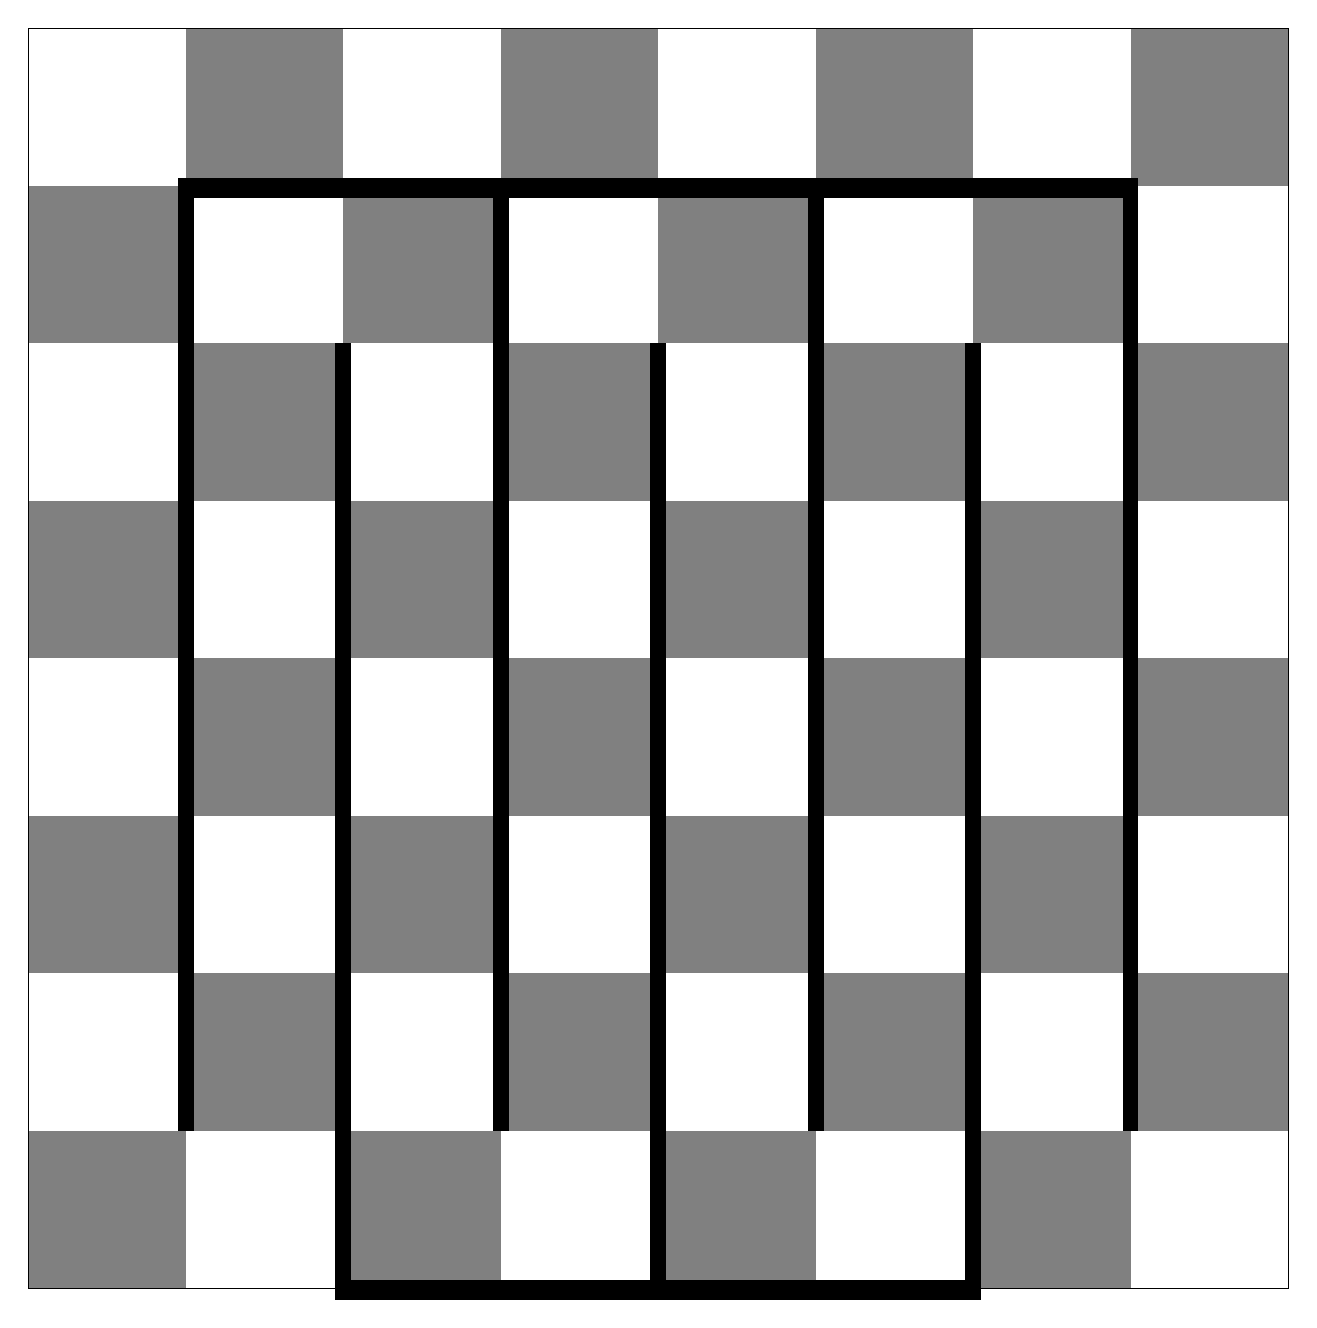
\begin{tikzpicture}[scale=2]
    \foreach \i in {0,1,...,7} {
      \foreach \j in {0,1,...,7} {
        \pgfmathtruncatemacro{\shade}{mod(\i+\j,2)}
        \ifnum\shade=0
          \fill[gray] (\i,\j) rectangle ++(1,1);
        \else
          \fill[white] (\i,\j) rectangle ++(1,1);
        \fi
      }
    }

    \draw (0,0) rectangle (8,8);
\foreach \i in {1,3,5,7} {
  \fill[black] (\i-.05,1) rectangle (\i+.05,7);
  
}
\foreach \i in {1,3,5}{\fill[black] (\i+1-.05,0) rectangle (\i+1.05,6);}
\fill[black] (1-.05,7-.075) rectangle (7.05,7.05);
\fill[black] (2-.05,-.075) rectangle (6.05,.05);
  \end{tikzpicture}


\end{document}